% multi: https://texblog.org/2012/12/21/multi-column-and-multi-row-cells-in-latex-tables/

% Mit pdflatex mindestens 2mal uebersetzen und Ergebnis mit einem pdf-Viewer betrachten
%\documentclass{beamer}
% https://en.wikibooks.org/wiki/LaTeX/Colors
\documentclass[usenames,dvipsnames,handout]{beamer}
%\usepackage[latin1]{inputenc}
%\usepackage[ngerman]{babel}
\usepackage[utf8]{inputenc}
\usepackage[ngerman]{babel} 
\usepackage{color}
\usepackage{multirow,array}
%\usepackage{multirow}
\usepackage{hyperref}
\usepackage{tikz}
\usetikzlibrary{shapes.geometric, arrows}
\usetikzlibrary{fit,arrows,calc,positioning}
% http://tex.stackexchange.com/questions/33231/how-to-change-the-color-of-a-block-within-a-custom-beamer-sty-theme-file
\usepackage{color}
\definecolor{mygreen}{cmyk}{0.82,0.11,1,0.25}
\usetheme[secheader]{Boadilla}
\newenvironment{variableblock}[3]{%
  \setbeamercolor{block body}{#2}
  \setbeamercolor{block title}{#3}
  \begin{block}{#1}}{\end{block}}


\begin{document}
\author[Dr. Mariana Nold]{Dr. Mariana Nold}
% \begin{center}
\institute[Institut für Soziologie]{ Institut für Soziologie,\\ Fakultät für Sozial- und Verhaltenswissenschaften,\\ Lehrstuhl für
 empirische Sozialforschung und Sozialstrukturanalyse}
% \end{center}
 \date{}
\title [Grundlagen des statistischen Testens]{Grundlagen des statistischen Testens}
\date{13. November 2017}
\begin{frame}
\maketitle

  \begin{figure}[ht]
 	\centering
 	      
\includegraphics[width=0.15\textwidth]{index.jpeg}
 	\end{figure}
\end{frame} 

\begin{frame}
  \frametitle{Übersicht}
  \tableofcontents
\end{frame}

\section{Ziel der heutigen Veranstaltung }
\begin{frame}{Ziel der heutigen Veranstaltung \dots}
ist es die folgenden Fragen beantworten zu können:
\begin{block}{Zielfragen für heute}
\begin{enumerate}
\item{Was bedeuten die Begriffe Nullhypothese und Forschungshypothese?}
\item{Welche der beiden Hypothesen kann man nachweisen?}
\item{Wie sind der $\alpha$-Fehler und der $\beta$-Fehler definiert?}
\item{Was ist das Signifikanzniveau bzw. die Irrtumswahrscheinlichkeit?}
\item{Was versteht man unter einer Teststatistik?}
\item{Welche Rolle spielt der kritische Wert?}
\item{Was versteht man unter einem p-Wert?}
%\item{}
%\item{Was versteht man unter der Teststärke?}
\end{enumerate}
\end{block}
\end{frame}
\section{Signifikanter Unterschied zwischen den Gruppen}
% https://stats.stackexchange.com/questions/3911/when-are-confidence-intervals-useful

\begin{frame}{Die Grundidee des Signifikanztests}
\begin{itemize}
\item{Wir werden uns heute an einem Beispiel   ansehen, welcher Logik der klassische
Signifikanztest folgt. }\pause
\item{Unser Fokus liegt  hierbei weniger auf die mathematischen
Zusammenhänge, als vielmehr auf die wissenschaftstheoretische Legitimation dieser Vorgehensweise.}\pause
\item{Die Darstellung orientiert sich an den  lesenswerten Kapiteln 
\begin{itemize}
\item{\textit{4.3.1: Die Grundidee von Signifikanztests (+Vorwort, ab S. 136)}}
\item{\textit{4.3.2: Die Praxis von Signifikanztests am Beispiel des Testens von Mittelwertunterschieden (nur bis S. 151)}}
\item{\textit{4.3.2 Problem statistischen Testens}}
\end{itemize} aus dem Buch ``Statistik-Eine Einführung für Sozialwissenschaftler'' von Ludwig-Mayerhofer, Liebeskind, Geißler,
(im Folgenden mit LMLG abgekürzt.)
 }
\end{itemize}
% Wichtig: Abschnitt 4.3.6
\end{frame}
\subsection{Kann das Zufall sein?}


\begin{frame}{Gibt es einen Unterschied hinsichtlich eines Merkmals in zwei Gruppen?}
Ich  werde heute anhand eines Beispiels darstellen, was die Behauptung:\\ `` Der Unterschied 
 hinsichtlich eines Merkmals in zwei Gruppen ist signifikant'' bedeutet. Zu dem Beispiel habe ich keine Daten.
 \begin{block}{Reales Beispiel: Kann das Zufall sein?}
 In einer Einrichtung zur stationären Drogenfreien Therapie, hat ein Klient den Eindruck zu wenig Gulasch auf 
 seinem Teller zu haben. Er fragt jemand vom Personal, ob es Zufall sein kann, dass er und
 die anderen Klientinnen und Klienten, wenn es Gulasch gibt, immer nur zwei oder drei Stücke Fleisch auf dem Teller
 haben und die Mitarbeiterinnen und Mitarbeiter deutlich mehr.
 \end{block}
\end{frame}

\begin{frame}{Die Vermutung des Klienten}
\begin{itemize}
\item{Er hat die Vermutung, dass der Koch, der das Gulasch ausgibt tiefer schöpft, wenn ein Mitarbeiter oder eine Mitarbeiterin 
vor ihm steht.}\pause
\item{Wenn seine Vermutung zutrifft, dann sind es zwei Unterschiedliche Zufallsmechanismen.}\pause
\item{In diesem Fall, kann es vorkommen, dass eine Klientin bzw. ein Klient mehr Fleisch auf dem Teller
hat als ein Mitarbeiter oder eine Mitarbeiterin, \textbf{aber nach Wahrscheinlichkeit, haben die Angestellten mehr
Fleisch auf dem Teller, als die die dort eine Therapie machen?}}\pause
\item{Die Vermutung kann daher überprüft werden, indem man die Mengen an Fleisch vergleicht.}\pause
\item{Dabei sind verschieden Vorgehensweisen denkbar.}
\end{itemize}
\end{frame}

\begin{frame}{Kann der Sachverhalt mit statistischen Methoden geklärt werden?}
\begin{itemize}
\item{Im Prinzip nicht, denn es bleibt immer eine Unsicherheit. Man kann allerdings
die Unsicherheit quantifizieren.}\pause
\item{Desto mehr empirische Information uns vorliegt, desto sichere wird unsere Aussage. Mit anderen Worten:
Desto länger wird diesen Ausgabeprozess beobachten, desto werden wir in der Beurteilung der Vermutung 
}\pause
\item{Dabei gilt die Annahme, dass der Prozess sich nicht verändert. Das bedeute, wir gehen davon aus, dass das Modell mit dem wir arbeiten,
die ganze Zeit über gleicher Maßen gut passt.}\pause
\end{itemize}
\end{frame}

\begin{frame}{Ein geeignetes Modell I}
Wir brauchen ein Modell, um auf der Modellebene arbeiten zu können.
\begin{itemize}
\item{Das Modell ist folgendes: Ich bezeichne mit der Zufallsvariable $X,$ die Menge Fleisch auf den Tellern
der Klientinnen und Klienten und mit $Y$ entsprechen die Menge Fleisch auf den Tellern der 
Mitarbeiterinnen und Mitarbeiter. }
\item{In einem Gedankenexperiment, wird der Prozess ein Jahr lang beobachtet.}
\item{Immer, wenn es Gulasch wird aus jeder Gruppe eine einfache Zufallsstichprobe  gezogen. Die am Ende erreichten Stichprobenumfänge
werden mit $n_{1}$ (für $X$) und $n_{2}$ (für $Y$) bezeichnet.}
\item{In der List der Klienten und Klientinnen sehen die Daten formal so aus:
$x_{1},x_{2},\dots,x_{n_{1}},$ dabei entspricht jedes $x_{i}$ einer beobachteten Zahl. }
\end{itemize}
\end{frame}

\begin{frame}{Ein geeignetes Modell II}
\begin{itemize}
\item{In formaler Schreibweise haben wir $n_{1}$ Realisation der Zufallsvariable $X_{1}$ und $n_{2}$ 
Realisation der Zufallsvariable $Y.$}
\item{Ich mache jetzt die folgenden Modellnahmen
$X_{i}$ iid wie 
\begin{equation}\label{eq1}
X \sim N(\mu_{X},\sigma_{X})
\end{equation}
und $Y_{i}$ iid wie
\begin{equation}\label{eq2}
Y \sim N(\mu_{Y},\sigma_{Y}).
\end{equation}
}
%\item{}
\end{itemize}
\end{frame}
\subsection{Das Modell grafisch}

\begin{frame}{Bitte fassen Sie die Folgenden Bilder in Worte}
\begin{itemize}
\item{Die folgenden Bilder zeigen in gelb die Modell-Dichte für $X$ und in grün
die Modell-Dichte für $Y.$}
\item{In den grafisch dargestellten Modellen gilt jeweils: $\sigma_{X}=\sigma_{Y}$}
\item{Der Überlappungsbereich ist je in Weinrot dargestellt.}
\item{Wenn die Modell so der Realität entsprechen würden, was würde das bedeuten?}
\end{itemize}
\end{frame}

\begin{frame}{$\mu_{X}=200,$ $\mu_{Y}=300,$ $\sigma_{X}=\sigma_{Y}=25$}
  \begin{figure}[ht]
 	\centering
 	      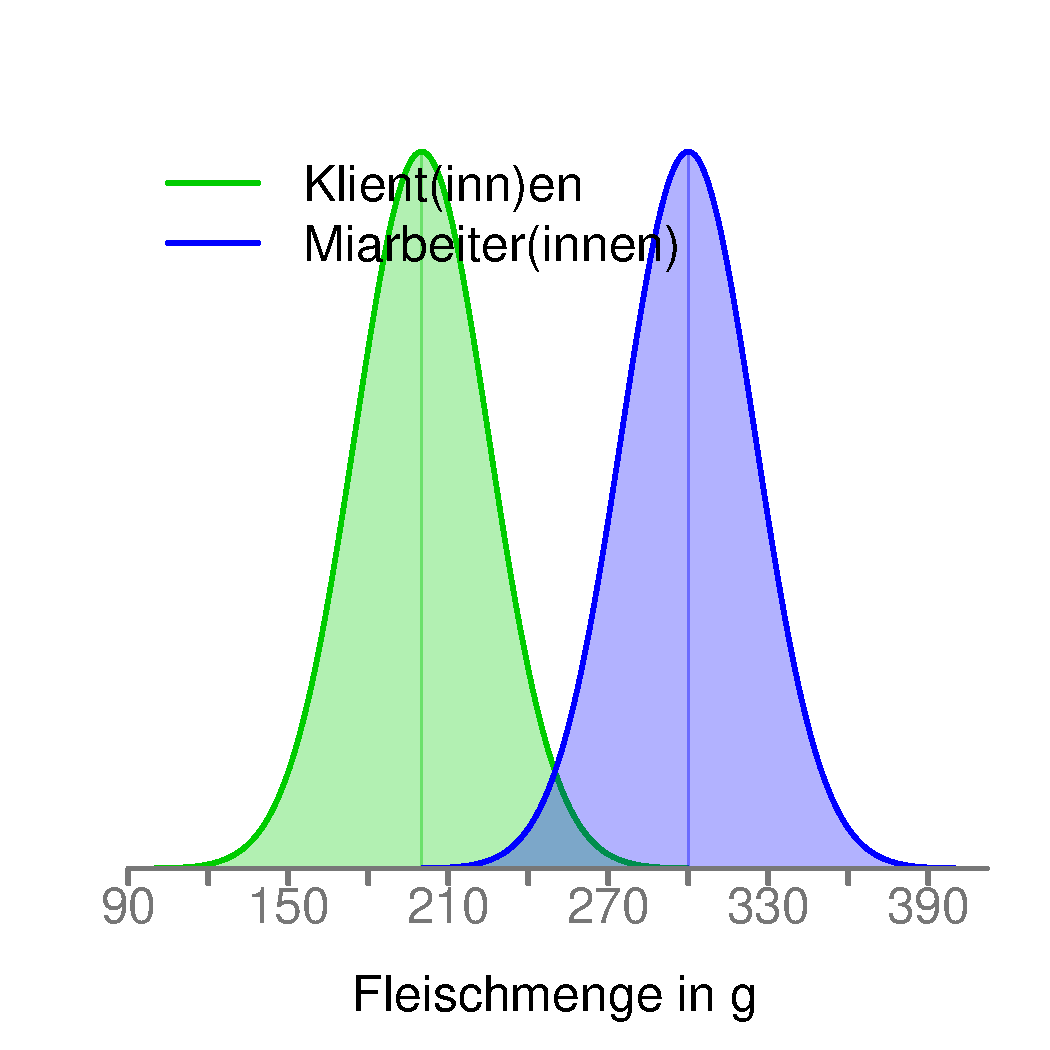
\includegraphics[width=0.65\textwidth]{mx200my300sd25.pdf}%{overlap3.pdf}
 	\end{figure}
%pdf("overlap3.pdf")
\end{frame}
%
\begin{frame}{$\mu_{X}=200,$ $\mu_{Y}=300,$ $\sigma_{X}=\sigma_{Y}=40$}
  \begin{figure}[ht]
 	\centering
 	      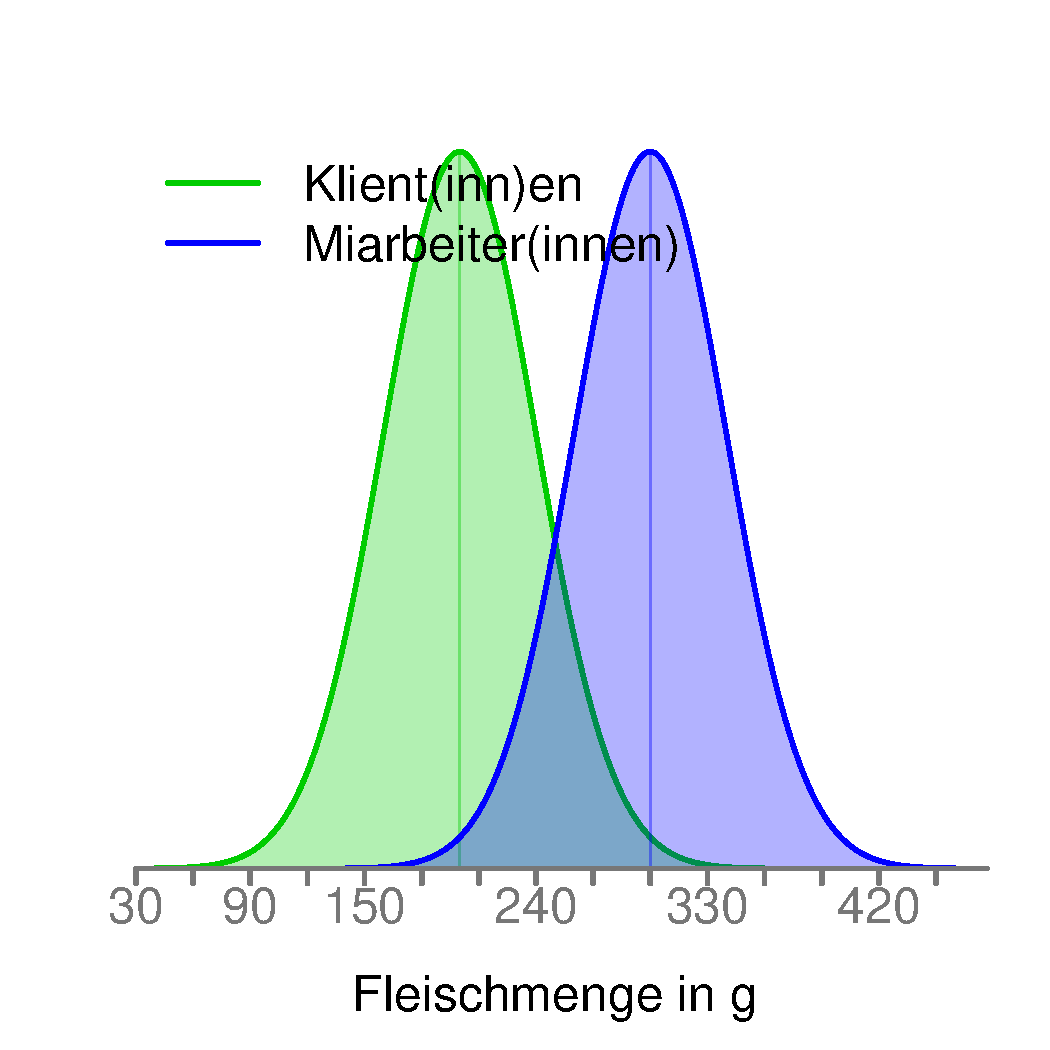
\includegraphics[width=0.65\textwidth]{mx200my300sd40.pdf}
 	\end{figure}
%pdf("overlap3.pdf")
\end{frame}
%
\begin{frame}{$\mu_{X}=200,$ $\mu_{Y}=300,$ $\sigma_{X}=\sigma_{Y}=60$}
  \begin{figure}[ht]
 	\centering
 	      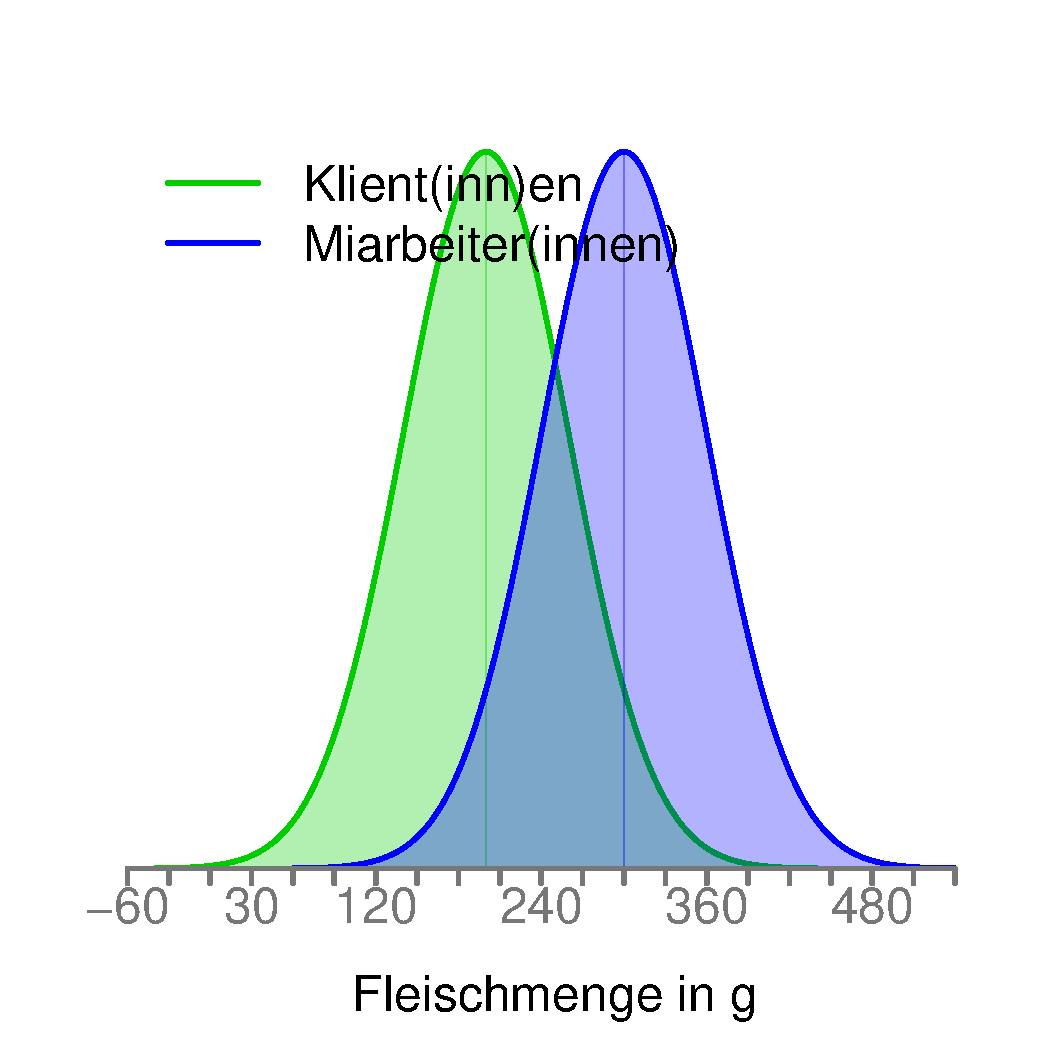
\includegraphics[width=0.65\textwidth]{mx200my300sd60.pdf}
 	\end{figure}
%pdf("overlap3.pdf")
\end{frame}
%
\begin{frame}{$\mu_{X}=200,$ $\mu_{Y}=300,$ $\sigma_{X}=\sigma_{Y}=80$}
  \begin{figure}[ht]
 	\centering
 	      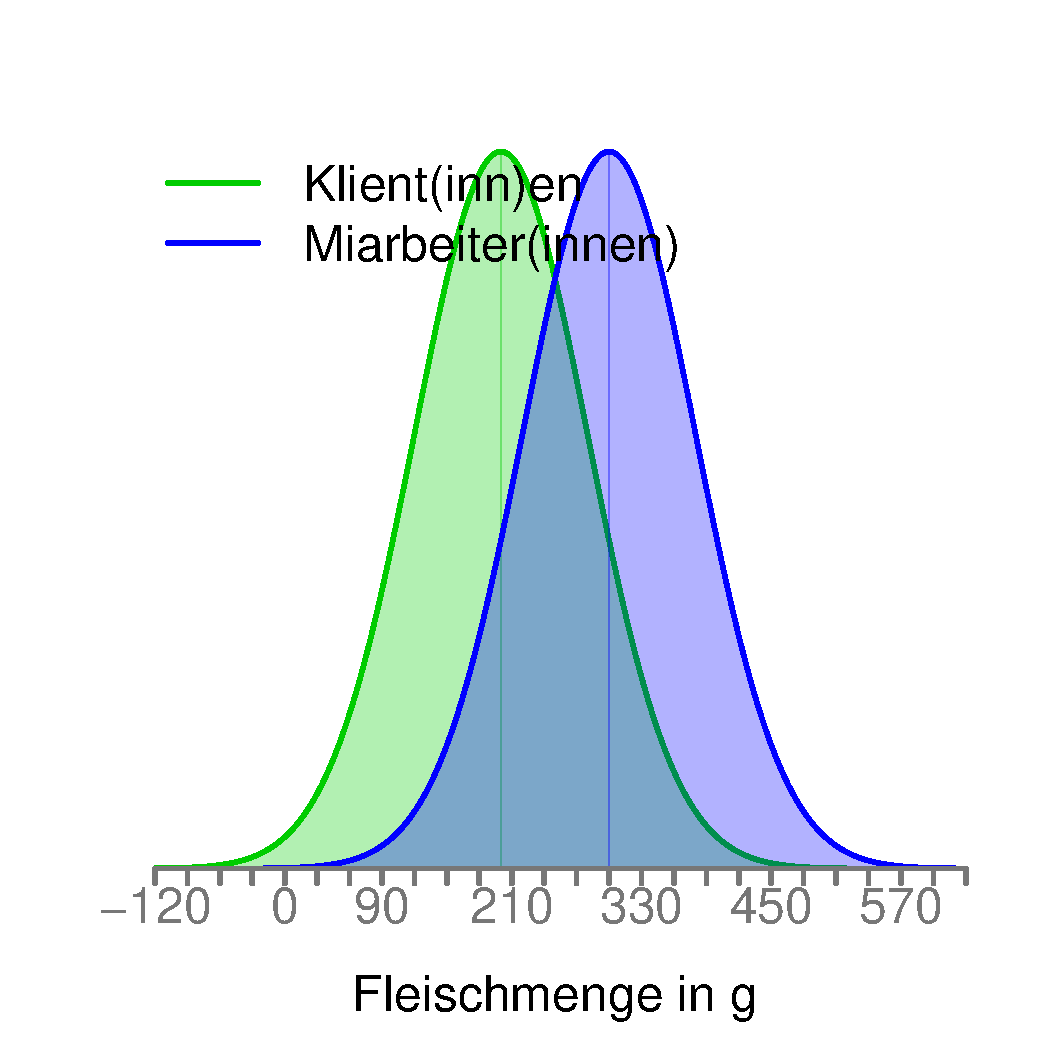
\includegraphics[width=0.65\textwidth]{mx200my300sd80.pdf}
 	\end{figure}
%pdf("overlap3.pdf")
\end{frame}
%
\begin{frame}{$\mu_{X}=220,$ $\mu_{Y}=280,$ $\sigma_{X}=\sigma_{Y}=40$}
  \begin{figure}[ht]
 	\centering
 	      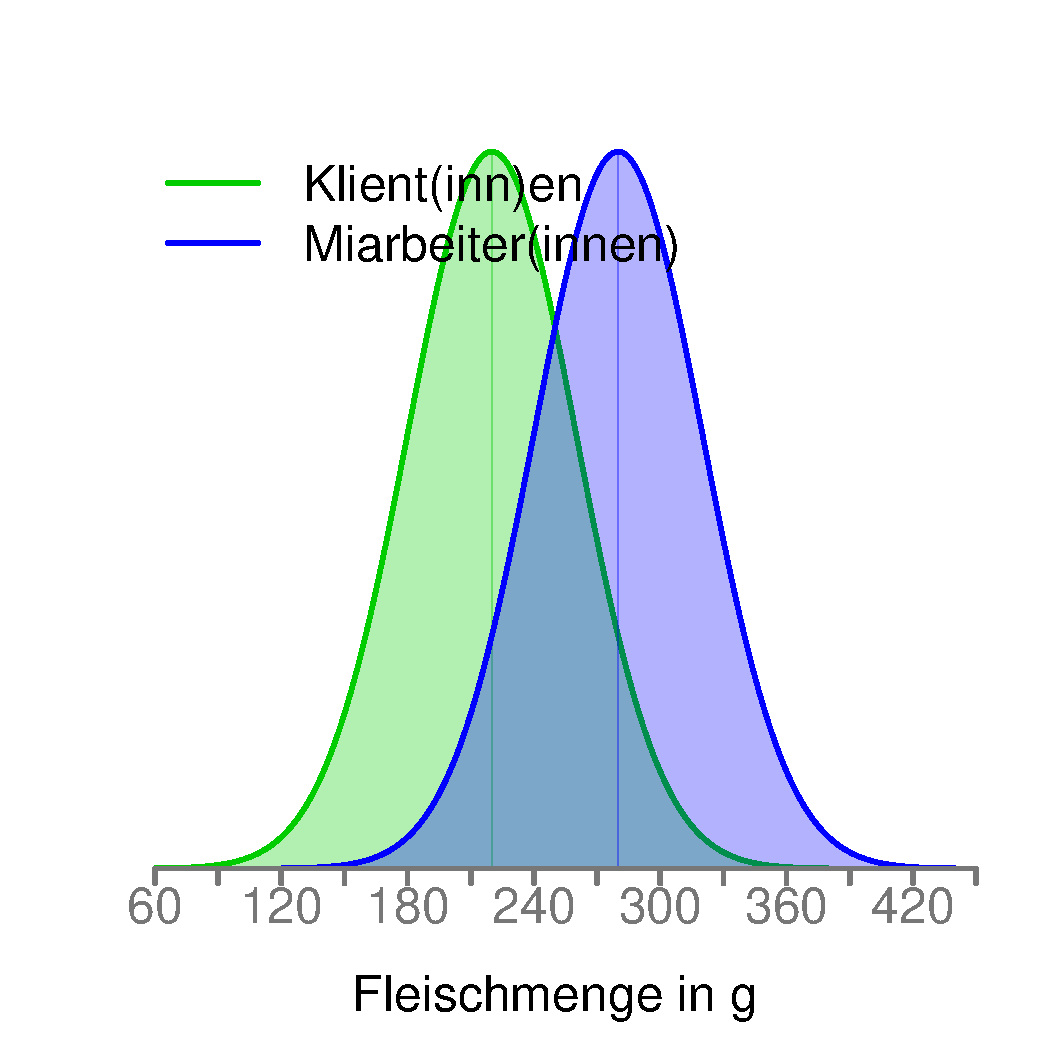
\includegraphics[width=0.65\textwidth]{mx220my280sd40.pdf}
 	\end{figure}
%pdf("overlap3.pdf")
\end{frame}
\subsection{Die Grundidee des Signifikanztest}
\begin{frame}{Die Hypothese}
Wenn man die Vermutung als statistische Hypothese formuliert, lautet sie
$$
\mu_{X} < \mu_{Y}.
$$
Die Gegenvermutung lautet:
$$
\mu_{X} \geq \mu_{Y}.
$$
Ich nenne die Gegenvermutung im Folgenden Nullhypothese und die Vermutung Forschungshypothese (bzw. Alternativhypothese).

\end{frame}

\begin{frame}{Die Grundidee des Signifikanztest I}
\begin{itemize}
\item{Beim klassischen statistischen Testen, gehen wir davon aus, dass die Nullhypothese gilt.}\pause
\item{Die Nullhypothese ist das Gegenteil von der Vermutung die wir nachweisen möchten. Wir gehen also davon aus,
dass die Hypothese die wir nachweisen möchten nicht gilt.}\pause
\item{Die Vorgehensweise erinnert an die Unschuldsvermutung im deutschen Strafrecht aus Perspektive der Staatsanalschaft.}\pause
\item{Die Staatsanwaltschaft möchte die Schuld nachweisen, die Schuld entspricht dann der Forschungshypothese.
Sie geht von der Unschuld auch, die Unschuld ist die Nullhypothese.}
\end{itemize}
\end{frame}

\begin{frame}{Die Grundidee des Signifikanztest II (vgl. LMLG S. 139)}
\begin{itemize}
\item{Unsere Nullhypothese (Unschuldsvermutung) ist $\mu_{X} \geq \mu_{Y}.$ Wir gehen davon aus, dass sie die Realität
beschreibt.}\pause
\item{Wenn wir nun in der Stichprobe tatsächlich ein Ergebnis beobachten, das im Lichte der Nullhypothese unwahrscheinlich ist, so spricht
das \textit{gegen} diese hypothetische Annahme. }\pause
\item{Wir schließen dann, dass die Nullhypothese nicht haltbar ist, mit Bezug auf die Daten.}\pause
\item{Wenn die Nullhypothese nicht haltbar ist, dann wird sie abgelehnt. }
\item{Wenn wir die Hypothese $\mu_{X} \geq \mu_{Y}$ ablehnen, dann folgt logische das wir $\mu_{X} < \mu_{Y}$ nachgewiesen haben.}
\end{itemize}
\end{frame}


\begin{frame}{Ein Irrtum ist möglich, \dots}
genauer zwei Irrtümer sind möglich:
\begin{itemize}
\item[1)]{Wir lehnen die Nullhypothese ab, obwohl sie wahr ist. Man nennt diesen Fehler $\alpha$-Fehler oder Fehler 1. Art.}
\item[2)]{Wir behalten die Nullhypothese bei, obwohl sie falsch ist. Man nennt diesen Fehler $\beta$-Fehler oder Fehler 2. Art.}
\end{itemize}
\begin{block}{Vorsicht!}
Es ist nicht möglich die Nullhypothese nachzuweisen. Man kann sie nur beibehalten, weil nicht genug empirische 
Evidenz dagegen spricht.
\end{block}
\end{frame}

\begin{frame}{Was bedeutet signifikant?}
\begin{itemize}
\item{Signifikant ist gleichbedeutend mit über-zufällig.}
\item{Wenn die Daten so stark gegen die Nullhypothese sprechen, dass man sich nicht mehr vorstellen kann,
dass die Nullhypothese war ist und nur durch Zufall ein so stark widersprüchliches Ergebnis zu Stande kommt.}\pause
\item{Als Maß dafür zu entscheiden, ob das Ergebnis über-zufällig ist, dient der $\alpha$-Fehler.}\pause
\item{Damit der Test gültig ist, muss man vor der Durchführung des Tests festlegen, wie groß
der $\alpha$-Fehler höchstens sein darf. Üblich Werte sind $1\%,$ $5\%$ oder $10\%.$}
\end{itemize}
%$\alpha$-Fehler wird kontrolliert
\end{frame}

\begin{frame}{Irrtumswahrscheinlichkeit als Schutz von $H_{0}$}

\begin{itemize}
\item{Wie gehen davon aus, dass der Koch den Klientinnen und Klienten mindestens so viel Fleisch auf den Teller
schöpft, wie den Mitarbeiterinnen und Mitarbeitern. In Formalsprache: $$H_{0}: \mu_{X} \geq \mu_{Y}$$ }\pause
\item{In Analogie: Das ist entspricht der Unschuldsvermutung}\pause
\item{Wir schützen diese Nullhypothese bzw. Unschuldsvermutung durch das Signifikanzniveau.}\pause
\item{Wir können nicht ausschließen, dass wir einen Irrtum begehen. Wir können aber festlegen,
dass die Wahrscheinlichkeit des $\alpha$-Fehlers höchstens $5\%$ beträgt.}\pause
\end{itemize}
\end{frame}

\begin{frame}{Die Bedeutung des Signifikanzniveaus}
\begin{itemize}
\item{Der Begriff Signifikanzniveau ist gleichbedeutend mit dem Begriff Irrtumswahrscheinlichkeit.}\pause
\item{Desto niedriger das Signifikanzniveau (bzw. die Irrtumswahrscheinlichkeit), desto stärker müssen 
die Daten gegen die Nullhypothese sprechen damit sie verworfen wird.}\pause
\item{Sehr häufig wählt man das Signifikanzniveau $5\%.$}\pause
\item{Wenn wir noch mehr Sicherheit möchten, um möglichst sicher zu sein, dass wir nicht 
$H_{0}$ verwerfen, obwohl es in Wirklichkeit gilt, dann können wir auch ein Signifikanzniveau von $1\%$ wählen.}
\end{itemize}
\end{frame}

\begin{frame}{Nullhypothese verwerfen}
Wenn die Analyse der Daten, also signifikant gegen die Nullhypothese spricht mit einem Signifikanzniveau von 
$5\%,$ dann können wir dem Koch sagen:
\begin{block}{Inhaltliche Bedeutung}
Lieber Koch, es kann sein, dass $H_{0}: \mu_{X} \geq \mu_{Y}$ gilt, aber es ist sehr unwahrscheinlich, dass wir 
unter Gültigkeit von $H_{0}$ die Daten so wie sind beobachten können. Wir gehen davon aus, dass es kein Zufall ist und verwerfen
die Nullhypothese. Die Wahrscheinlichkeit für einen Irrtum beträgt $5\%.$
\end{block}
\end{frame}
\section{Die Teststatistik und die Testentscheidung}

\begin{frame}{Wie kann man entscheiden, ab wann man $H_{0}$ verwirft?}
\begin{itemize}
\item{Für einen (klassischen) parametrischen statistischen Test, braucht man ein Teststatistik.}\pause
\item{Ich möchte Ihnen heute eine Teststatistik vorstellen, um zu zeigen, wie der Test abläuft.}\pause
\item{Es gibt viele statistische Tests, sie brauchen die entsprechenden Teststatistiken nicht zu kennen. }\pause
\item{Für die Herleitung unserer Teststatistik brauchen wir die Modellannahme der Normalverteilung,
also $X \sim N(\mu_{X},\sigma_{X})$ und $Y \sim N(\mu_{Y},\sigma_{Y}).$ 
Wir nehmen an $X_{i}$ iid wie $X$ und $Y_{i}$ iid wie Y.}\pause
\item{Im Folgenden mache ich die zusätzliche Annahme $\sigma_{X}=\sigma_{Y}.$}
\end{itemize}
\end{frame}

\begin{frame}{Die zusätzliche Annahme $\sigma_{X}=\sigma_{Y}.$}
\begin{itemize}
\item{Je nachdem ob man diese Annahme macht oder nicht, gibt es zwei unterschiedliche Tests,
die auch auf unterschiedlichen Teststatistiken beruhen.}\pause
\item{Ich mache diese Annahme jetzt, um anhand der entsprechenden Teststatistik, zu zeigen,
wie man darüber entscheidet, ob man die Nullhypothese beibehält oder nicht.}\pause
\item{Es gibt auch einen stat. Test mit der Nullhypothese  $H_{0}: \sigma_{X}=\sigma_{Y}.$ }\pause
\item{Manchmal rechnet man zuerst diesen Test um dann zu entscheiden, ob man von der Gleichheit
der Standardabweichungen ausgehen kann oder nicht. }
\item{Natürlich ist auch hier ein Irrtum möglich.}
\end{itemize}
\end{frame}

\subsection{Die Teststatistik}
% Je ein Besipiel für
\begin{frame}{Unsere  Teststatistik}
Leseempfehlung:  (vglm LMLG S. 141- 152)
\begin{itemize}
\item{Die Nullhypothese $H_{0}$ bzw. die Forschungshypothese $H_{1}$ beinhalten eine Beziehung
zwischen den Erwartungswerten der Normalverteilung $\mu_{X}$ und $\mu_{Y}.$}\pause
\item{Wir hatten schon im letzten Semester gesehen, dass das arithmetische Mittel $\bar{X}$ bzw. $\bar{Y}$
ein guter Schätzer für $\mu_{X}$ bzw $\mu_{Y}$ ist.}\pause
\item{Mit den Gesetzen der Wahrscheinlichkeitstheorie lässt sich auch nachweisen, dass das arithmetische Mittel
als Schätzer für den Erwartungswert bei normalverteilten Daten eine hohe Güte hat.}\pause
%\item{Die Nullhypothese lautet: $$H_{0}:  \mu_{X} \geq \mu_{Y}$$ Gleichbedeutend damit ist: $$H_{0}:  \mu_{X} - \mu_{Y} \geq 0$$}
\end{itemize}
\end{frame}

\begin{frame}{Die Teststatistik entwickeln I}
Die Nullhypothese lautet: $$H_{0}:  \mu_{X} \geq \mu_{Y}$$ Gleichbedeutend damit ist: $$H_{0}:  \mu_{X} - \mu_{Y} \geq 0$$
Aus den gerade genannten Gründen ist die Differenz der Mittelwerte 
$$\bar{X}-\bar{Y}$$ gut geeignet um die Differenz der Modellparameter zu schätzen.
\end{frame}

\begin{frame}{Die Teststatistik entwickeln II}
\begin{itemize}
\item{Wir werden also aus den Daten $Z:=\bar{X}-\bar{Y}$ berechnen und auf das Ergebnis dieser Rechnung unsere Entscheidung über die Ablehnung
bzw. Beibehaltung der Nullhypothese stützen.}\pause
\item{Wir müssen dafür wissen, wie sich die Zufallsvariable $Z$ verhält, denn wir müssen wissen, welche Werte von $Z$ gegen die Nullhypothese
sprechen und auch wie stark sie dagegen sprechen.}\pause
\item{Ein Problem dabei ist, dass unsere Nullhypothese ein ganzes Intervall abdeckst. Wir ersetzen die Nullhypothese
für den Moment durch $\tilde{H}_{0}: \mu_{X} = \mu_{Y}$ bzw. analog $\tilde{H}_{0}:  \mu_{X} - \mu_{Y} = 0$}\pause
\item{Im Klartext bedeutet die modifizierte Nullhypothese, dass wir von völlig identischen Verteilungen der Fleischmengen pro Portion Gulasch ausgehen.}
\end{itemize}
\end{frame}

\begin{frame}{Die modifizierte Nullhypothese grafisch}
\begin{figure}[ht]
 	\centering
 	      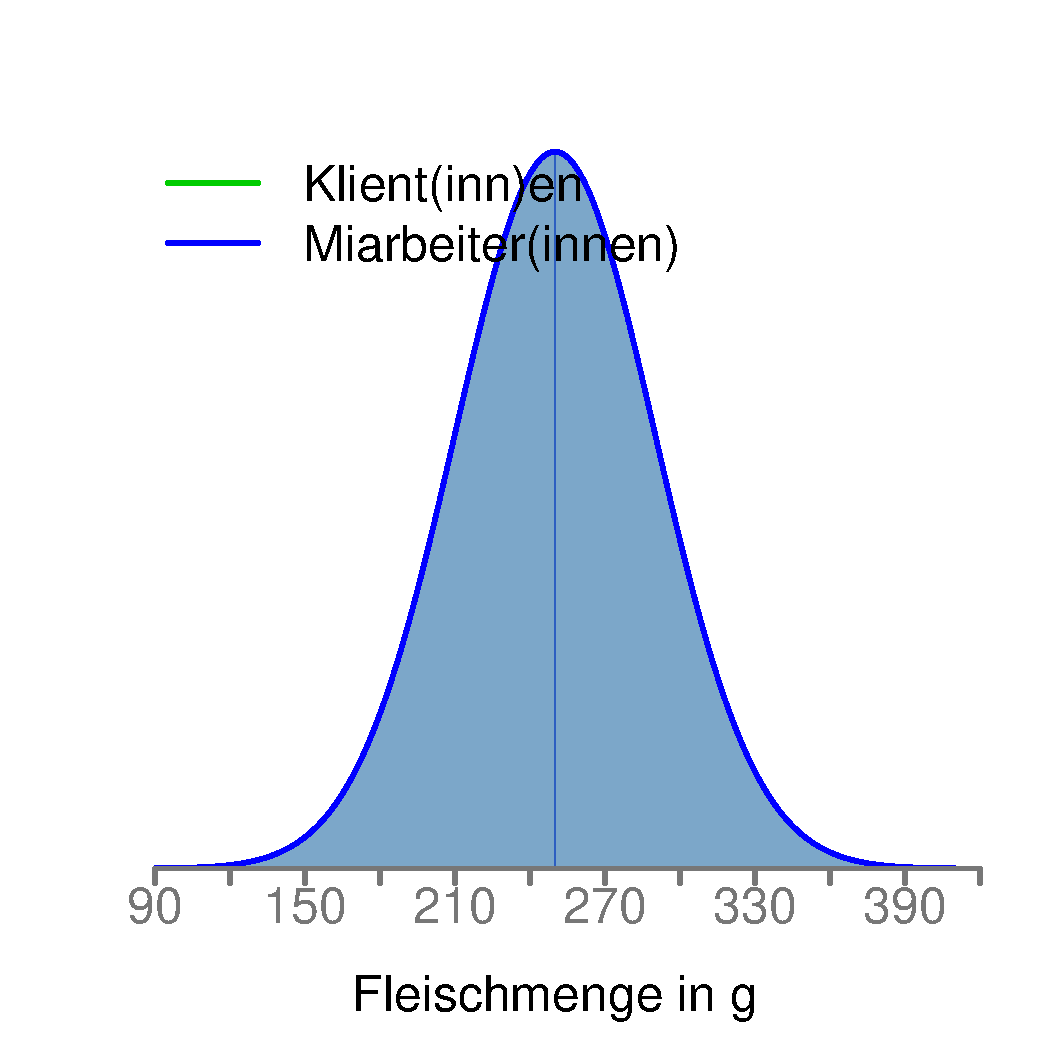
\includegraphics[width=0.65\textwidth]{nullhyp.pdf}
 	\end{figure}
\end{frame}

\begin{frame}{Wir gehen davon aus, dass die Nullhypothese zutrifft\dots}
\dots also davon, dass der Schöpfmechanismus beim Gulasch Schöpfen sich in den beiden Personengruppen gar nicht unterscheidet.
$$Z:=\bar{X}-\bar{Y}$$
\begin{itemize}
\item{Ich  simuliere die Datenerhebung . In der Simulation, wird die Fleischmenge von je $100$ Personen der 
beiden  Gruppen erfragt. In der Simulation gehe ich davon aus, dass kein Unterschied in der Verteilung der Fleischmenge besteht.}\pause
\item{Ich gehe davon aus, dass die erwarte Fleischmenge $250$ g beträgt, mit einer Standartabweichung von $40$ g. (Das entspricht der Abbildung auf der vorigen
Folie)} 
\end{itemize}
\end{frame}

\begin{frame}{Die Verteilung der Teststatistik $Z:=\bar{X}-\bar{Y}$}

\begin{itemize}
\item{Wir haben jetzt Daten, von $10$ Personen jeder Gruppe, wir berechnen jeweils den Mittelwert.}\pause
\item{Die mittlere Fleischmenge $\bar{x}$ ergibt sich zu $252.1$ g.}\pause
\item{Die mittlere Fleischmenge $\bar{y}$ ergibt sich zu $247.8$ g.}\pause
\item{Wir beobachten daher $z=\bar{x}-\bar{y}=4.3$ g.}\pause
\item{Finden Sie dass ein Unterschied von $4.3$ g als Hinweis darauf gesehen werden kann, dass der Koch unfair schöpft?}\pause
\item{Welche Werte würden dafür sprechen, dass der Koch unfair schöpft? Werte die größer oder kleiner sind als Null?}\pause
\item{Um wie viel muss der Wert unter Null liegen, dass sie sagen würden: ``Das kann kein Zufall sein.''?}
%\item{Welche Werte für $Z$ erwarten Sie?}
%\item{Erwarten Sie Werte, die Nahe bei Null sind oder Werte die von Null weit entfernt sind?}\pause
\end{itemize}
\end{frame}
%[1] -14.39033
%> x[47]
%[1] 237.6495
%> y[47]
%[1] 252.0399
\begin{frame}{Wir wiederholen das Experiment}
\begin{itemize}
\item{Wir stellen uns vor, dass wir einen weiteren Monat die Gulasch-Ausgabe beobachten. Wieder gilt die Nullhypothese. Der Koch schöpft
also gerecht.}\pause
\item{Wenn wir die Daten simulieren, dann wissen wir, dass der Koch fair schöpft. In der Realität beobachten wir einfach die 
Daten und wir wissen nicht, ob die Nullhypothese gilt.}\pause
\item{Die mittlere Fleischmenge $\bar{x}$ ergibt sich zu $237.6$ g.}\pause
\item{Die mittlere Fleischmenge $\bar{y}$ ergibt sich zu $252.0$ g.}\pause
\item{Wir beobachten daher $z=\bar{x}-\bar{y}=-14.4$ g.}\pause
\item{Wenn Sie nicht wüssten, dass die Daten unter Gültigkeit der Nullhypothese entstanden sind, wie würden sie diesen Wert beurteilen?}
\end{itemize}
\end{frame}

\begin{frame}{Ein kritischer Wert wird gebraucht}
\begin{itemize}
\item{Wir haben gesehen, auch, wenn die Nullhypothese gilt, kann es passieren, dass $Z$ Werte annimmt, die deutlich 
unter Null liegen und uns nahe legen, zu glauben, dass der Koch unfair schöpft.}\pause
\item{Wenn wir dann die Nullhypothese verwerfen, begehen wir den Fehler 1. Art ($\alpha$-Fehler)}\pause
\item{Für diesen Fehler hatten wir vereinbart, dass er einen Irrtumswahrscheinlichkeit von $5\%$ nicht übersteigen soll.}\pause
\item{Wir müssen den kritischen Wert also so wählen, dass die Wahrscheinlichkeit die Nullhypothese abzulehnen, wenn der Koch
in Wirklichkeit fair ist, höchsten $5\%$ beträgt.}
\end{itemize}
\end{frame}

\begin{frame}{Der kritische Wert ist $k:=-9.3$}
\begin{itemize}
\item{Der Wert, der die Eigenschaft hat, in unserem Beispiel, dass die Irrtumswahrscheinlichkeit gleich $5\%$ beträgt ist $-9.3$}\pause
\item{In Worten: Unter der Annahmen dass der Koch gerecht schöpft die die Wahrscheinlichkeit, dass bei je $10$ Portionen
Gulasch pro Gruppe, die Differenz der Mittelwerte kleiner als $-9.3$ ist, höchstens $5\%$}\pause
\item{Was sie verstehen sollten ist: }
\begin{itemize}
\item{Durch die Irrtumswahrscheinlichkeit ist der kritische Wert festgelegt.}
\item{Sie brauchen ihn nicht bestimmen zu können.}
\item{Sie sollten verstehen, welche Bedeutung er hat.}
\end{itemize}
\end{itemize}
\end{frame}

\begin{frame}{Verteilung der Teststatistik $Z$}
\begin{figure}[ht]
 	\centering
 	      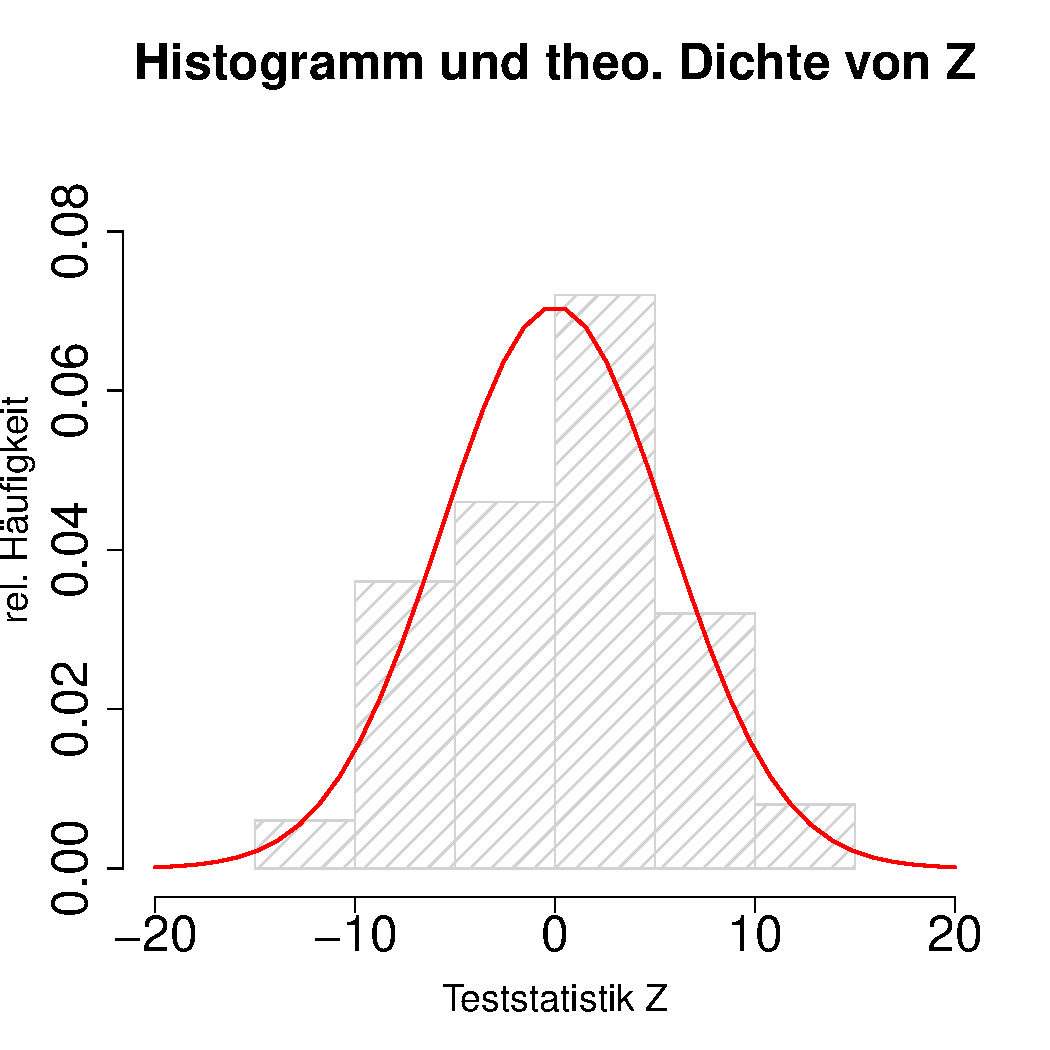
\includegraphics[width=0.65\textwidth]{distZ.pdf}
 	\end{figure}
\end{frame}

\begin{frame}{Verteilung der Teststatistik $Z$ und kritischer Wert $k$}
\begin{figure}[ht]
 	\centering
 	      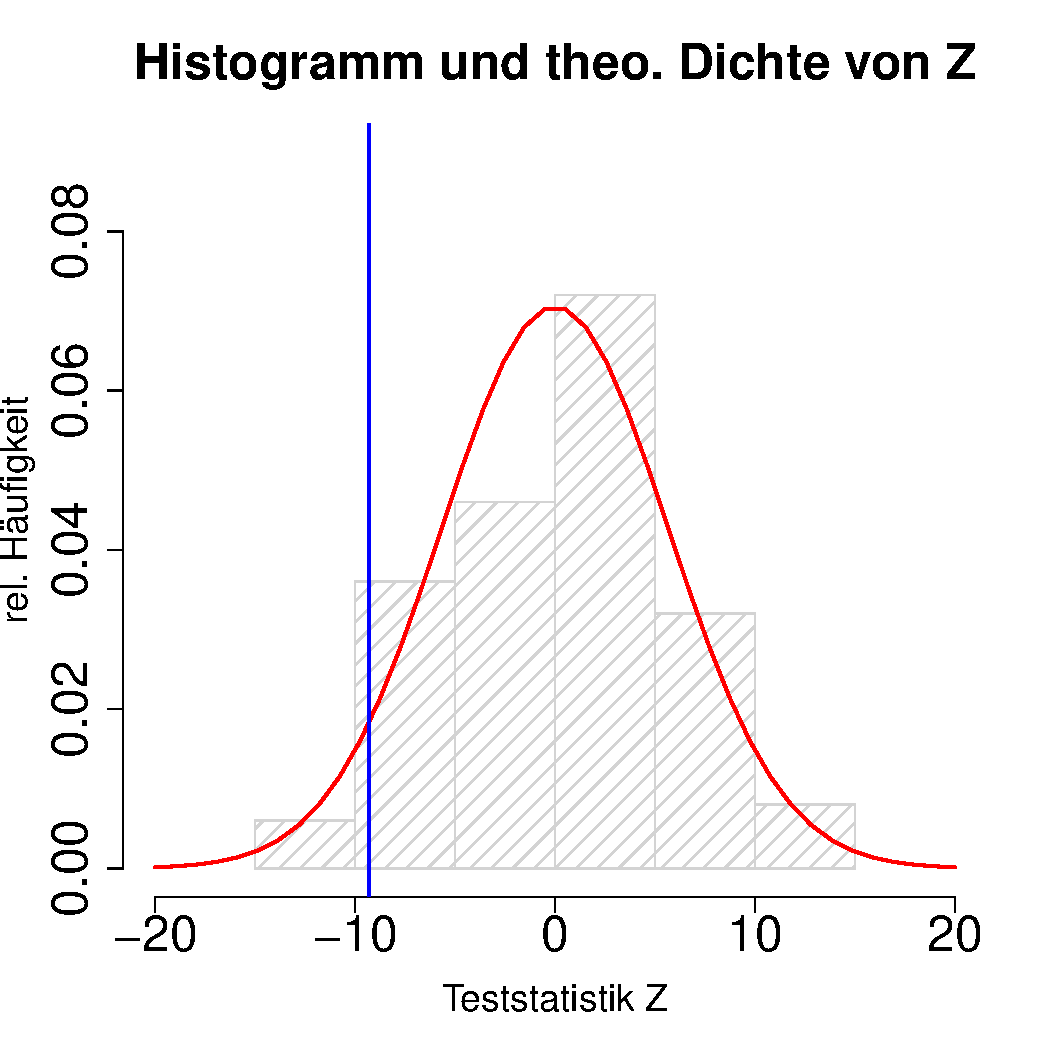
\includegraphics[width=0.65\textwidth]{distZ2.pdf}
 	\end{figure}
\end{frame}

\begin{frame}{Die Rolle der Stichprobenumfänge $n_{1}$ und $n_{2}.$}
\begin{itemize}
\item{Desto mehr Informationen man hat, desto kleiner sind die Unterschiede die der Test aufdecken kann.}\pause
\item{Nehmen wir an, die Differenz $\delta := \mu_{x}-\mu_{y}$ beträgt in Wirklichkeit nur $10g,$ dann braucht man
einen große Stichprobenumfänge $n_{1}$ und $n_{2}$ um diese kleine Differenz aufdecken zu können.}\pause
\item{Wenn $\delta$ einen Wert von $100$ g hat wird bereits ein kleiner Stichprobenumfang von z. B. $10$
Personen pro Gruppe zu einer Ablehnung der Nullhypothese führen.}\pause
\item{\colorbox{yellow}{Merksatz: Desto stärker die Nullhypothese verletzt ist,} 
\colorbox{yellow}{desto weniger empirische Information braucht man,}
\colorbox{yellow}{um die Forschungshypothese nachzuweisen.}}
\end{itemize}
\end{frame}

\begin{frame}{Von der modifizieren Nullhypothese zu Nullhypothese}
\end{frame}



\begin{frame}{ Gulasch-Beispiel}
Ein paar Anmerkungen: 
\begin{itemize}
\item{Die Nullhypothese und die Forschungshypothese sind in ihrer Bedeutung unterschiedlich.}
\item{Es gibt zwei Möglichkeiten sich zu irren: Den Fehler 1. Art und den Fehler 2. Art. Auch diese werden unterschiedlich
behandelt.}
\item{Der Fehler 1. Art wird a-priori festgelegt und durch ihn wird der kritische Wert  bestimmt.}
\item{Beruhend auf dem kritischen Wert können wir entscheiden, ob wir glauben, dass der Koch frair ist oder nicht. Wir wissen 
wir hoch die Wahrscheinlichkeit ist, ihn zu unrecht als ungerecht einzustufen.}
\item{Die Verteilung der Teststatistik $Z$ hängt von den Stichprobenumfängen $n_{1}$ und $n_{2}$ ab.}
\end{itemize}
\end{frame}

\begin{frame}{Zusammenfassung: statistisches Testen allgemein}
\begin{itemize}
\item[1)]{Wenn wir die Modellannahmen formuliert haben, und die Hypothesen aufgestellt, dann suchen wir nachdem Test, der für dieses Problem geeignet ist. Das Signifikanzniveau
wird festgelegt.}
\item[2)]{Dieser Test hat eine Teststatistik. Die Teststatistik, legt fest, welcher Wert aus den Daten berechnet wird, um die Testentscheidung zu treffen.}
\item[3)]{Durch die Festlegung der Irrtumswahrscheinlichkeit (=Signifikanzniveau) und der des Auswahl der Teststatistik, ergibt sich ein kritischer Wert. }
\item[4)]{Die Statistik-Software
berechnet diesen Wert und informiert uns darüber ob wir die Nullhypothese beibehalten, oder  ob sich die Forschungshypothese nachweisen lässt.}
\end{itemize}
\end{frame}

\subsection{Der Ablehnbereich und der p-Wert}

\section{Ausblick Übung: Häufige Testprobleme}% FT S. 433

\begin{frame}{Übung}
Wir werden für einige Testproblem die häufig auftreten die geeigneten Test auswählen, mit STATA rechnen und die Ergebnisse interpretieren.
Wir behandeln:
\begin{itemize}
\item{Approximative Binominaltest}% S.397, S405
\item{$\chi^{2}$ Unabhängigkeitstest}
\item{Test zu Lagealternativen im Ein- und Zwei-Stichprobenfall:}
\begin{itemize}
\item{Ein-Stichprobenfall: einfacher Gaußtest und  t-Test}% S. 437
\item{Zwei-Stichprobenfall (unabhängige Stichproben): doppelter Gauß- und t-Test, Welch-Test
 } % S. 457 ff
\end{itemize}
\end{itemize}
\end{frame}

%\begin{frame}{Ein andere Zufallsmechanismus beim Gulasch schöpfen?}
%\end{frame}
%\subsection{Binomial- und Normalverteilung}
%\begin{frame}{Der Inferenzschluss}
%\end{frame}
% Beispiel mit Menge Fleisch in der Suppe
%\subsection{Der Inferenzschluss}
% Wenn man Paramter schätzt, dann kann man Inferenzschluss ziehen
\end{document}

